\section{\texorpdfstring{\ttbar}{TTbar} Background}
\label{sec:bkg_tt}

The \ttbar process contributes about 21\,\% to the total background in our search. We rely on MC to model the process-specific kinematic properties. To that effect, we first verify that the simulation works well in dilepton events, and then correct the MC misidentification rate to match the one in data.

\subsection{Dilepton Studies}
The \ttbar control region is defined by exactly 2 opposite-sign opposite-flavor leptons ($e^\pm \mu^\mp$), at least 1 b-tagged jet above 30\,\GeV, and $\ST > 300\,\GeV$, where \ST is the scalar sum of the lepton transverse momenta, the transverse momenta of jets with $\pt \geq 30\,\GeV$ and $|\eta| \leq 2.4$, and \MET. We use this region to normalize the background prediction; the normalization factor is $0.80 \pm 0.01\stat$.

We also use this control region to derive weights in bins of $n_\textrm{jets}$ (see Fig.~\ref{fig:tt/NGOODJETS}). The corrections typically range between 1\,\% and 10\,\%. Note that, as we do not bin our signal regions in jet-related quantities, the impact of these weights on the results is neglibile. Still, as the $n_\textrm{jets}$ distribution was seen to be in disagreement, weights were applied to improve the general accuracy of the simulation.

\begin{figure}
\begin{center}
	\begin{subfigure}[b]{.7\textwidth}
		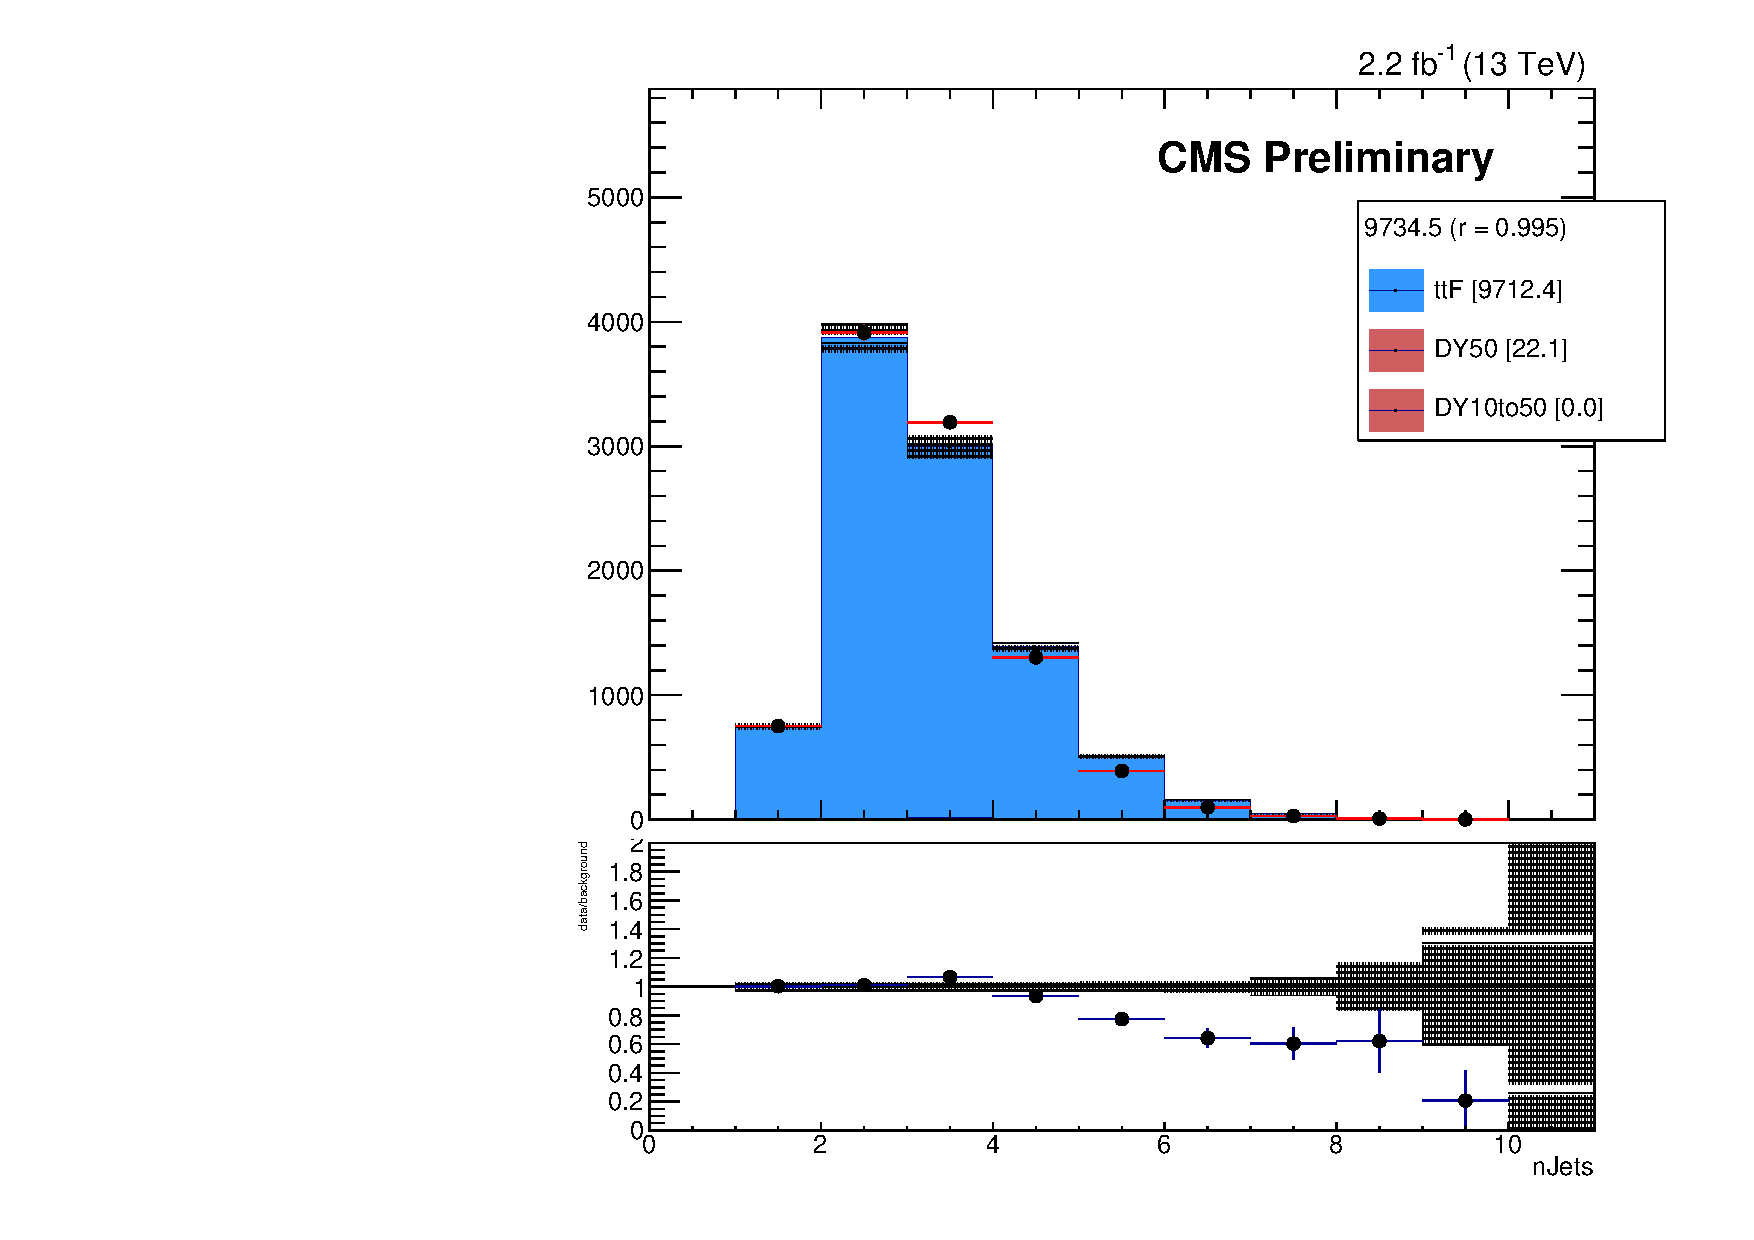
\includegraphics[width=\textwidth]{Background/bkg_tt/ttbar_NGOODJETS_STgt300_beforeWeights}
		\caption{$n_\textrm{jets}$ distribution before weights}
	\end{subfigure}
	\begin{subfigure}[b]{.7\textwidth}
		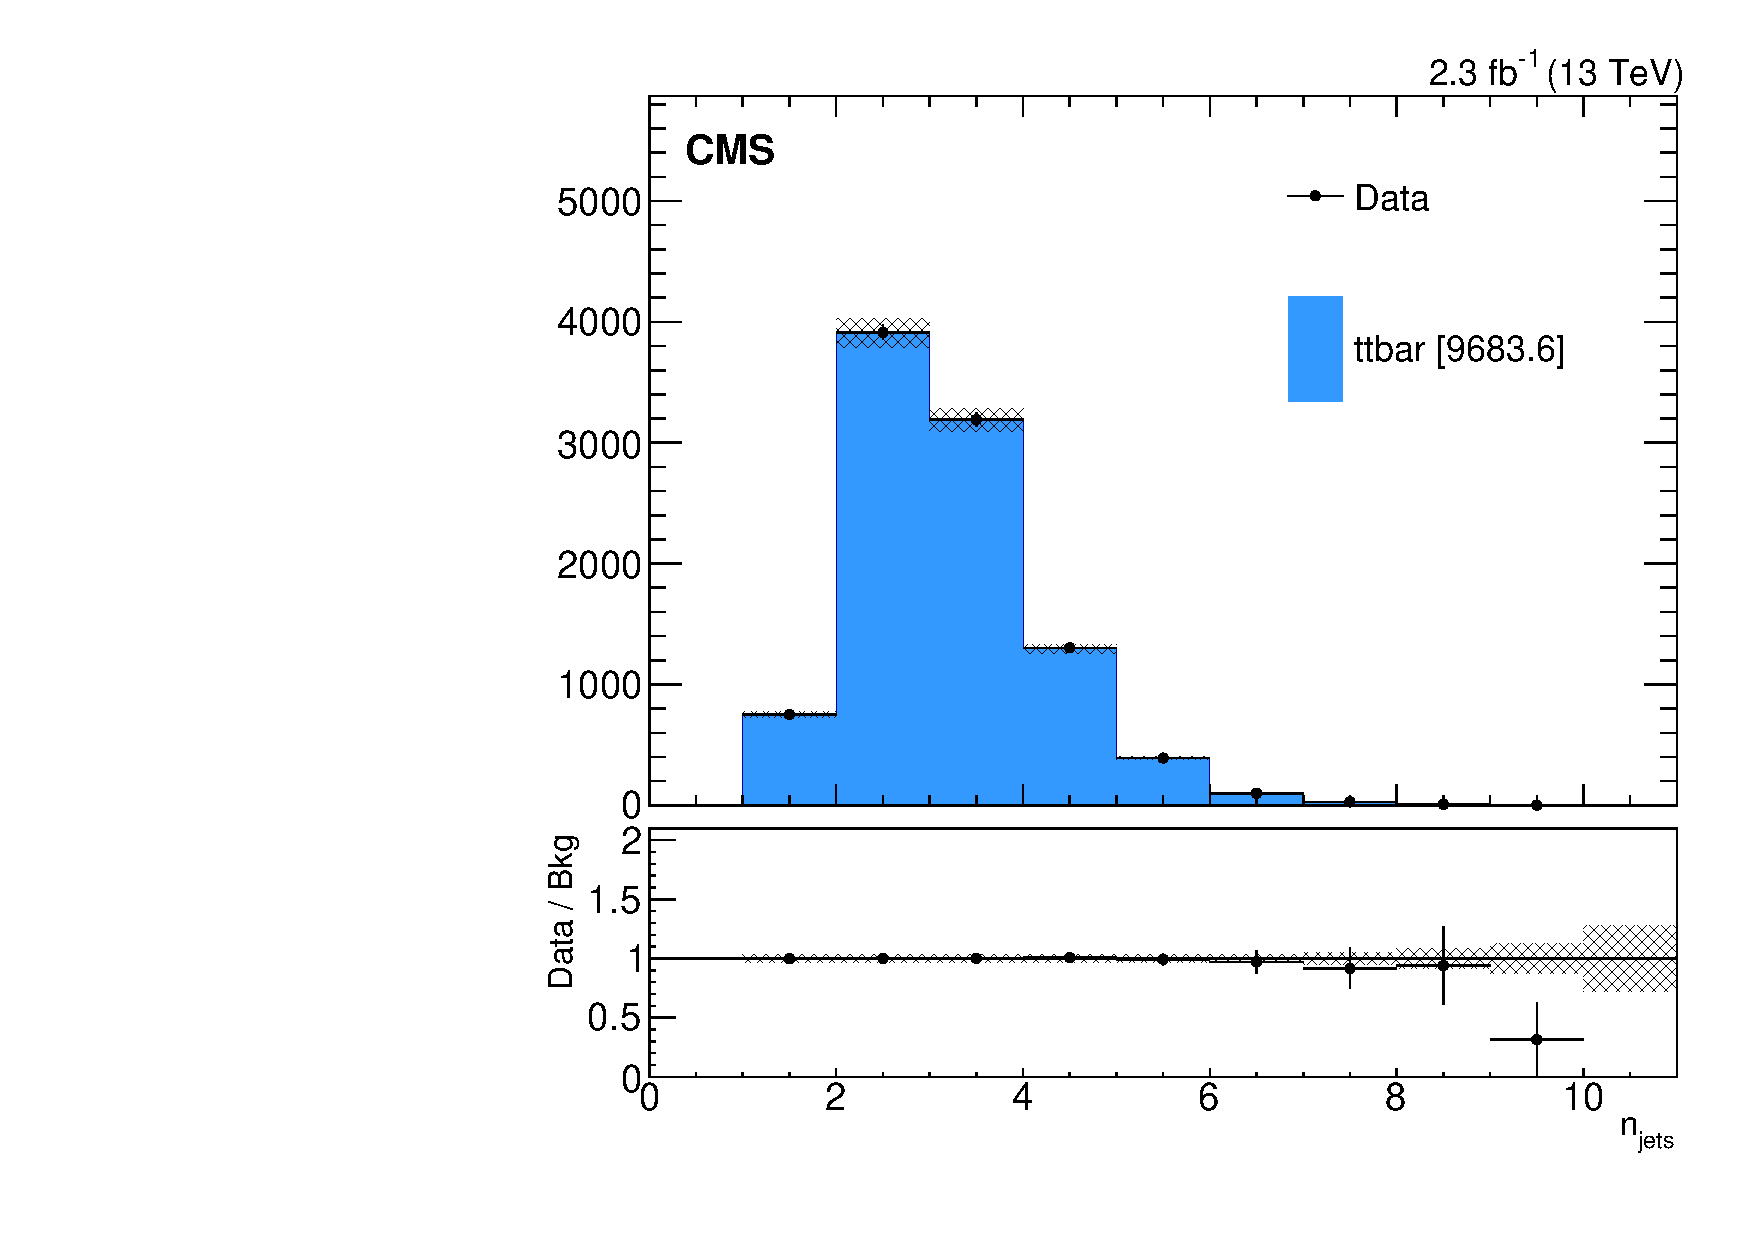
\includegraphics[width=\textwidth]{Background/bkg_tt/ttbar_NGOODJETS_STgt300_afterWeights}
		\caption{$n_\textrm{jets}$ distribution after weights}
	\end{subfigure}
	\caption{$n_\textrm{jets}$ distributions in \ttbar-dominated control region (last bin includes overflow). Uncertainties are statistical only. \fixme{style}
	\label{fig:tt/NGOODJETS}}
\end{center}
\end{figure}

The \MET and \ST distributions after normalization and weights are shown in Fig.~\ref{fig:tt/METST}.

\begin{figure}
\begin{center}
	\begin{subfigure}[b]{.7\textwidth}
		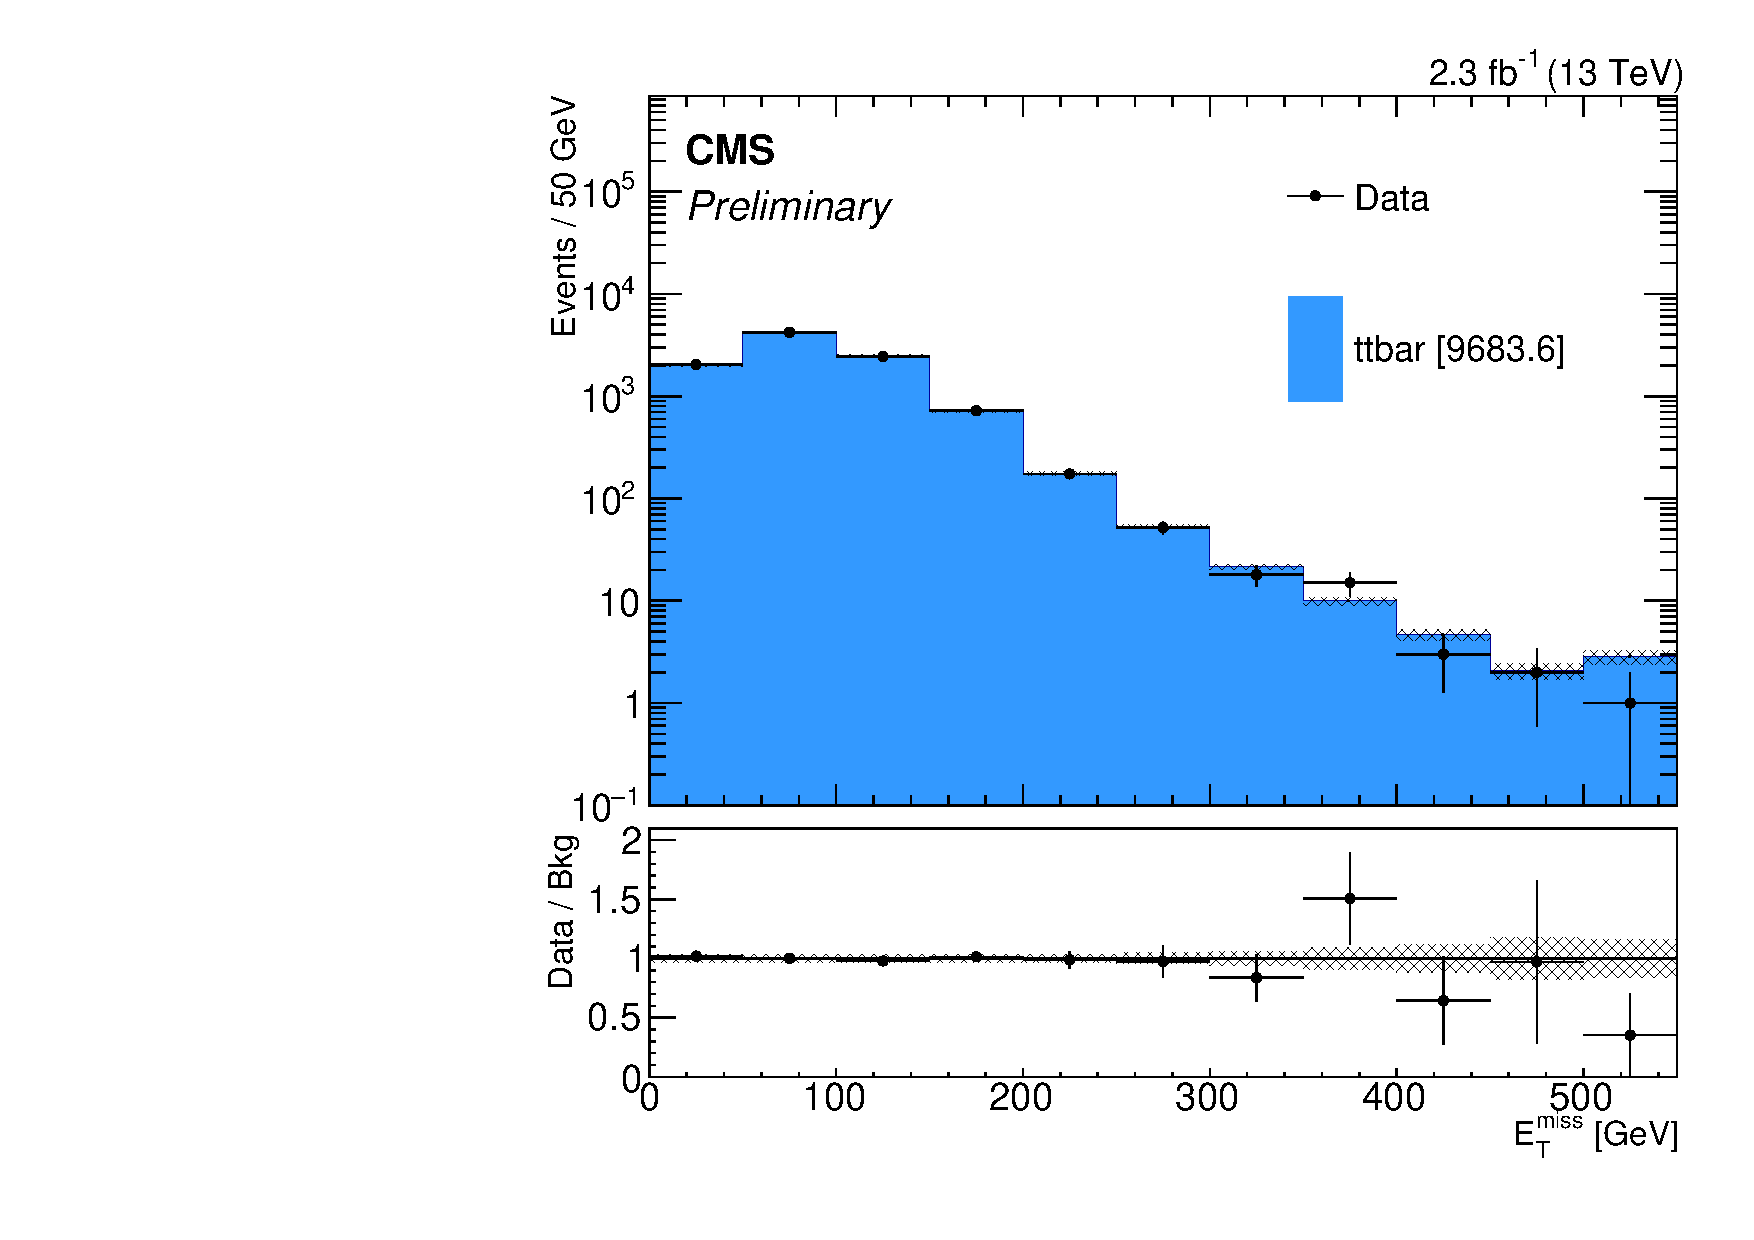
\includegraphics[width=\textwidth]{Background/bkg_tt/ttbar_MET_STgt300_afterWeights}
		\caption{\MET distribution}
	\end{subfigure}
	\begin{subfigure}[b]{.7\textwidth}
		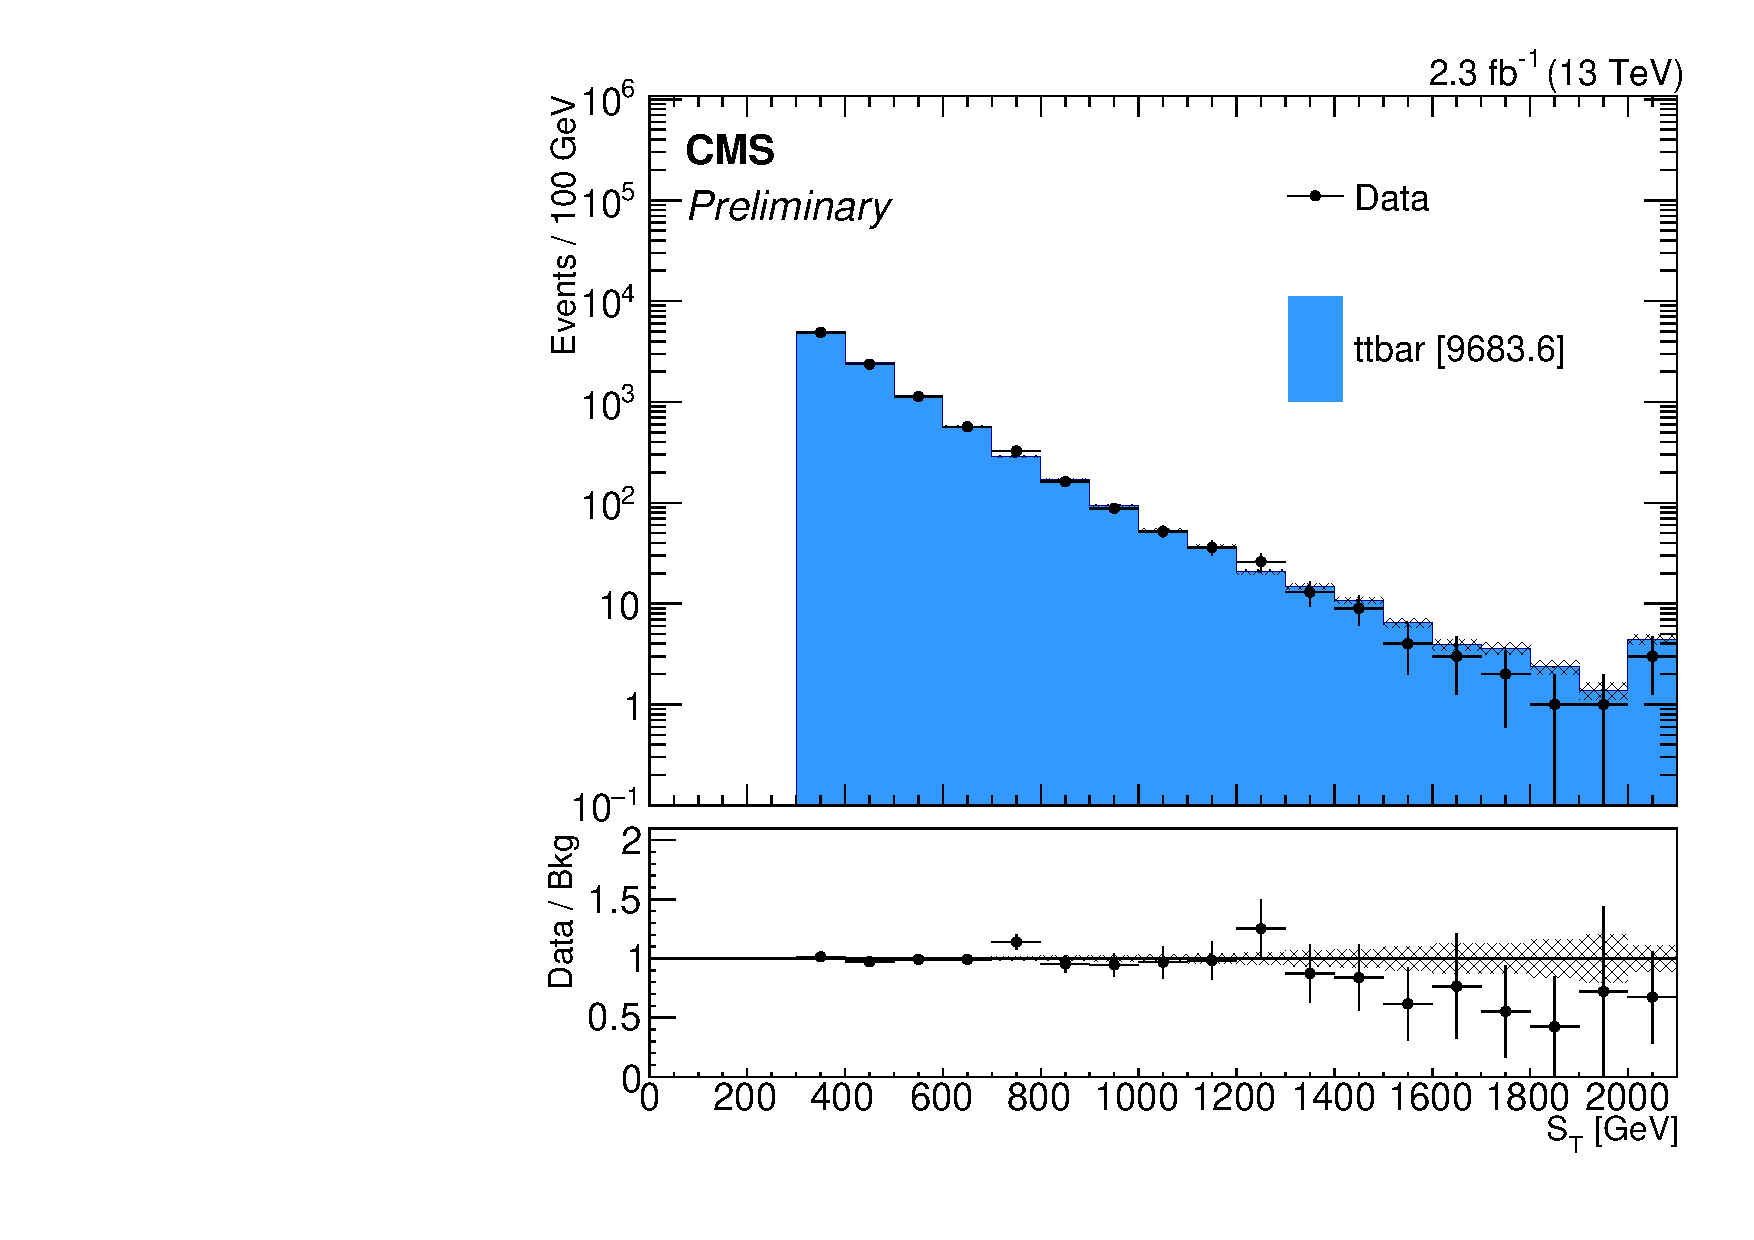
\includegraphics[width=\textwidth]{Background/bkg_tt/ttbar_ST_STgt300_afterWeights}
		\caption{\ST distribution}
	\end{subfigure}
	\caption{Kinematic distributions in \ttbar-dominated control region (last bin includes overflow). Uncertainties are statistical only.
	\label{fig:tt/METST}}
\end{center}
\end{figure}

\subsection{Trilepton Studies}
\label{sec:bkg_tt/trilepton}

Having established the validity of kinematic aspects of the \ttbar simulation using the dilepton (prompt) sample, we verify that also the rate at which the \ttbar MC produces trilepton events is in agreement with that rate in data. To this end, we measure the lepton misidentification rate in a sample dominated by semi-leptonic \ttbar decays. This sample is selected by requiring one tight muon with $\pt > 30\,\GeV$, 2 jets (from the other top quark), one additional b-tagged jet, and a non-prompt lepton which is most likely misidentified.

We find the \ttbar misidentification rate in data to be $1.5 \pm 0.5\stat$ times the one found in the \ttbar simulation. This indicates that the number of events with misidentified leptons is underpredicted in the \ttbar simulation. We thus use this ratio to correct the number of predicted trilepton events from \ttbar and apply a systematic uncertainty of 50\,\%.

\subsection{Dilepton + Track Studies}
\label{sec:bkg_tt/dilepton+track}

The prediction for the \Z + jets background (Sec.~\ref{sec:bkg_fakeLight}) uses isolated tracks as a handle to estimate the number of misidentified leptons from jets. However, some of these tracks may come from \ttbar + jets production, so that the two methods overlap. To avoid overpredicting the background in the \Z + jets method, the number of tracks as predicted by the \ttbar simulation is subtracted before calculating the track-based estimate. The reliability of this procedure depends on the accuracy of the track modeling in simulation.

We therefore verify that the number of tracks from \ttbar is predicted correctly, by comparing both the distributions of non-isolated tracks and of isolated tracks in the dilepton control region. While the former, shown in Fig.~\ref{fig:tt/trackNonIso}, agrees well with the data and gives us confidence in the general quality of the simulation, the latter shows disagreement in the bins with at least one isolated tracks (Fig.~\ref{fig:tt/trackIso}). We therefore scale the number of tracks from the \ttbar simulation by a factor of 1.5.

Considering both plots in Fig.~\ref{fig:tt/track} together suggests that the \ttbar simulation does not model the track isolation distribution distribution correctly. As the mismodeling of the \ttbar misidentification rate (Sec.~\ref{sec:bkg_tt/trilepton}) is quantitatively and qualitatively similar, it is likely that both discrepancies have a common cause in the simulation. We therefore apply the same systematic uncertainty (50\,\%) to the track prediction.

\begin{figure}
\begin{center}
	\begin{subfigure}[b]{.7\textwidth}
		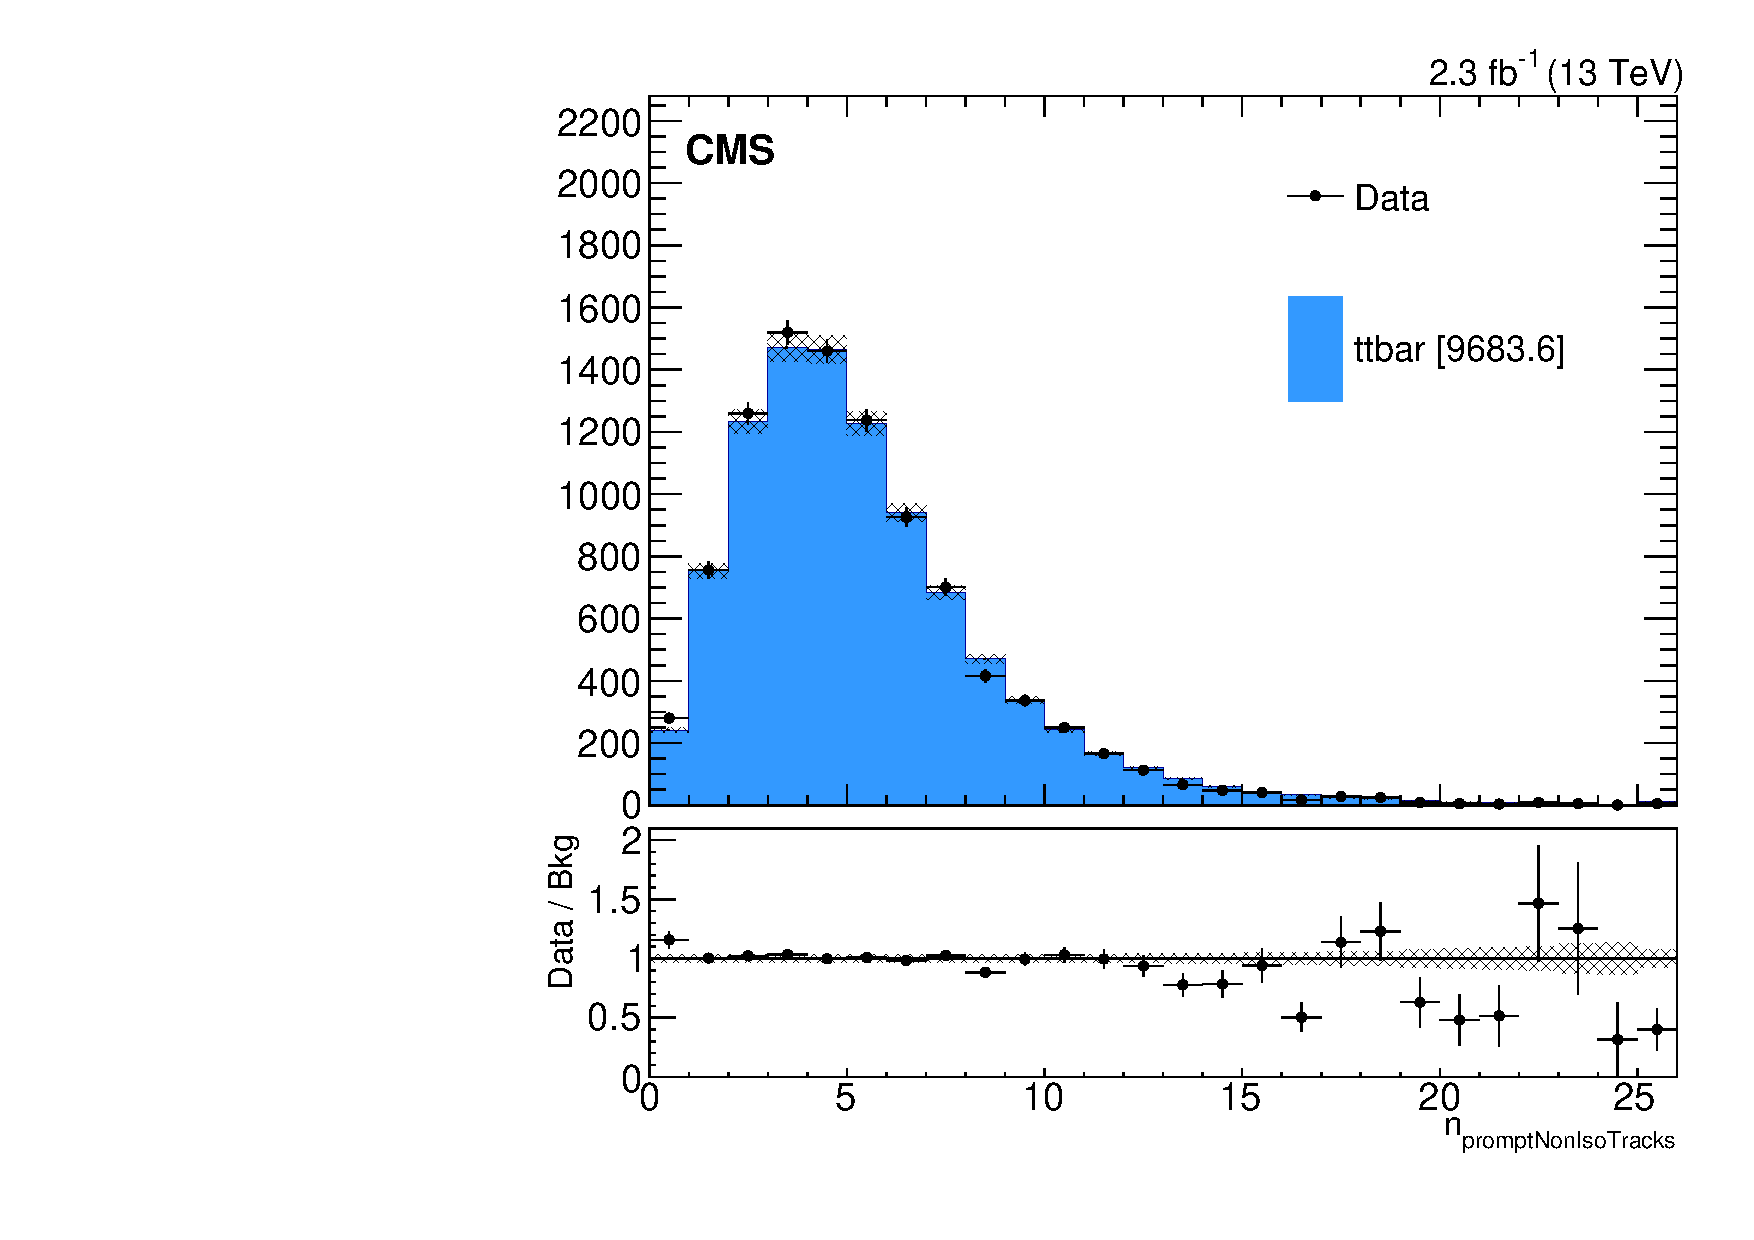
\includegraphics[width=\textwidth]{Background/bkg_tt/ttbar_NPROMPTNONISOINCLUSIVETRACKS7_STgt300}
		\caption{Number of non-isolated tracks \fixme{label}} \label{fig:tt/trackNonIso}
	\end{subfigure}
	\begin{subfigure}[b]{.7\textwidth}
		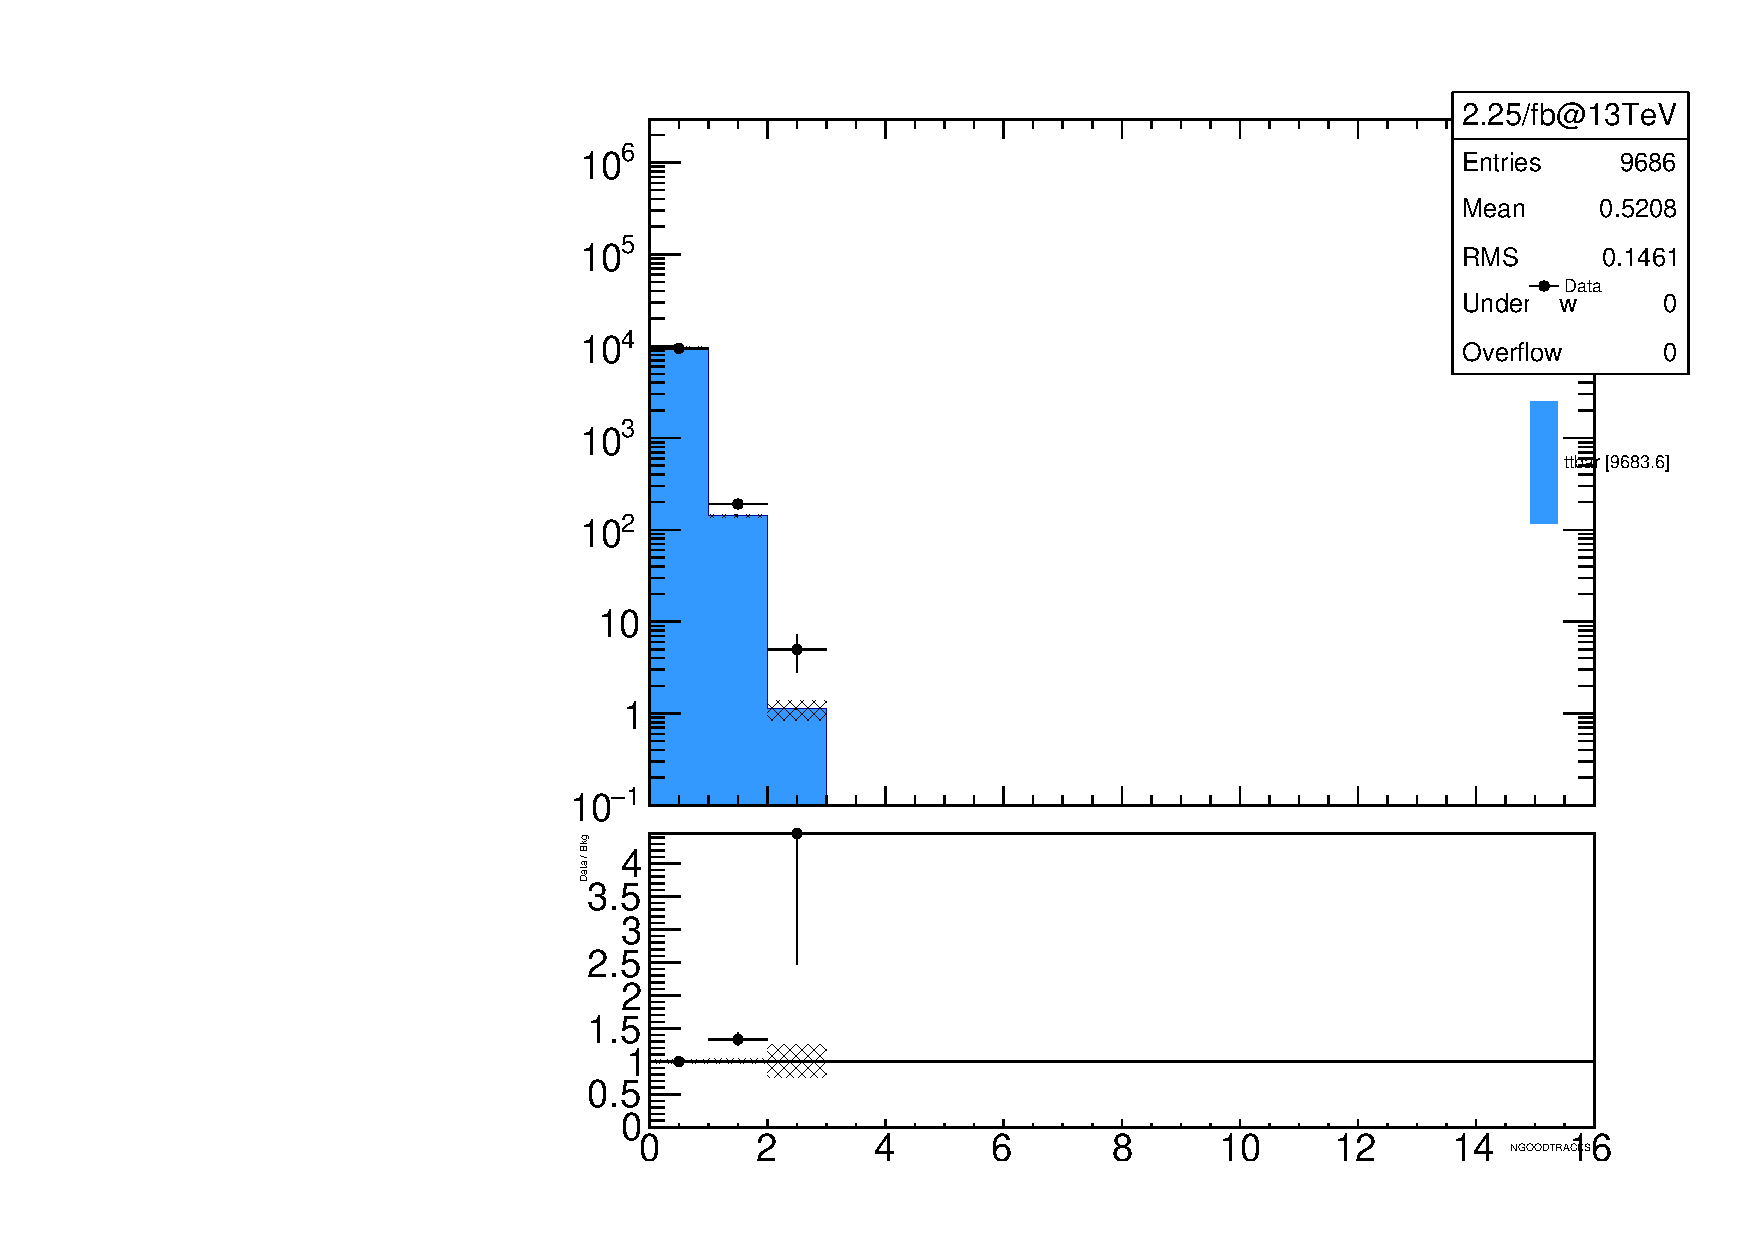
\includegraphics[width=\textwidth]{Background/bkg_tt/ttbar_NGOODTRACKS_STgt300}
		\caption{Number of isolated tracks \fixme{label, style}} \label{fig:tt/trackIso}
	\end{subfigure}
	\caption{Track distributions in \ttbar-dominated control region (last bin includes overflow). Uncertainties are statistical only.
	\label{fig:tt/track}}
\end{center}
\end{figure}

Further details on the \Z + jets background estimation can be found in Sec.~\ref{sec:bkg_fakeLight}.
